% =====================================================================
%  ch07.tex —— 第 7 章 示性类（原书 p.102–117）
%  §7.1 Čech 上同调  §7.2 H^1(M;A) 中的示性类  §7.3 H^2(M;A) 中的示性类
%  §7.4 H^3(M;A) 中的一个示性类  §7.5 分类空间
%  注意：原书 p.102 上半页属第 6 章末尾（定理 6.51、例 6.52、式 (6.53)），已由 ch06.tex 收录；
%        本 chunk 自 p.102 中段的第 7 章标题起译，保留 p.102 页锚点以覆盖页范围。
% =====================================================================

% [原文 p.102]
\chapter{示性类}

我们已经学过以 $\Z_2$ 和（或）$\Z$ 为系数的（上）同调群的基本知识，
下面看看它们如何出现在主 $G$-丛或向量丛的研究中。与丛相伴的上同调类称为示性类。

% [原文 p.103]
\section{Čech 上同调}

下面要处理的示性类，通常是在 Čech 上同调的框架里构造的，而这个框架我们还没介绍。
由于时间限制，我们只概述其想法。

设 $M$ 是一个空间，取 $M$ 的一个“足够细”的覆盖 $\{U_i\}$，
使得所有非空的交 $U_{i_1}\cap U_{i_2}\cap\cdots\cap U_{i_k}$ 都可缩。然后我们关联如下单纯复形：
\begin{itemize}
  \item 每个 $U_i$ 对应一个顶点 $v_i$；
  \item 每个非空交 $U_{ij}=U_i\cap U_j$ 对应一条边 $E(v_i,v_j)$；
  \item 每个非空交 $U_{ijk}=U_i\cap U_j\cap U_k$ 对应一个三角形 $T(v_i,v_j,v_k)$；
\end{itemize}
依此类推。

\begin{definition}{7.1}
与一个开覆盖相伴的单纯复形，称为该覆盖的神经（nerve）。
\end{definition}

\begin{definition}{7.2}
空间 $M$ 的 Čech 上同调，是 $M$ 的某个“足够细”覆盖的神经的单纯上同调。
\end{definition}

以 $A$ 为系数的 Čech $p$-上链 $c$，对一个覆盖 $\{U_i\}$ 而言，就是一列元素
\begin{equation}
c(i_0,i_1,\cdots,i_p)
\tag{7.1}
\end{equation}
它们在交换 $i_0,\dots,i_p$ 时反号；上边缘 $\delta$ 则和以前一样由下式给出：
\begin{equation}
(\delta c)(i_0,\cdots,i_{p+1})=\sum_{k=0}^{p+1}(-1)^k c(i_0,\dots,\hat{i}_k,\dots,i_{p+1}).
\tag{7.2}
\end{equation}

写出显式公式会很有用：
\begin{align}
(\delta a)(i,j) &= a(i)-a(j), \tag{7.3}\\
(\delta b)(i,j,k) &= b(j,k)-b(i,k)+b(i,j)=b(i,j)+b(j,k)+b(k,i), \tag{7.4}\\
(\delta c)(i,j,k,l) &= c(j,k,l)-c(i,k,l)+c(i,j,l)-c(i,j,k). \tag{7.5}
\end{align}

\takeaway{Čech 上同调把覆盖的神经当作单纯复形来计算：反称的 $p$-上链配上交错和上边缘 $\delta$，就得到不依赖覆盖细化的上同调群。}

\section{$H^1(M;A)$ 中的示性类}

\subsection{离散 Berry 相}

我们从次数 $p=1$ 的示性类开始。设 $A$ 是有限阿贝尔群，比如 $A=\Z_2$。
考虑 $M$ 上的主 $A$-丛 $A\to P\to M$。取足够细的覆盖。
它由 $U_{ij}$ 上把 $U_i\times A$ 与 $U_j\times A$ 粘起来的映射 $g_{ij}:U_{ij}\to A$ 指定，方式是
\begin{equation}
U_i\times A\ni(x,a)\mapsto(x,g_{ij}(x)+a)\in U_j\times A.
\tag{7.6}
\end{equation}

% [原文 p.104]
由于 $A$ 有限，$g_{ij}(x)$ 其实是一个常数，我们记作 $g_{ij}$。
在三重交 $U_{ijk}$ 上，我们从 $U_i$ 走到 $U_j$，再从 $U_j$ 走到 $U_k$，最后从 $U_k$ 回到 $U_i$。这给出的效果是
\begin{equation}
(x,a)\mapsto(x,g_{ij}a)\mapsto(x,g_{ij}g_{jk}a)\mapsto(x,g_{ij}g_{jk}g_{ki}a),
\tag{7.7}
\end{equation}
于是有
\begin{equation}
g_{ij}g_{jk}g_{ki}=1.
\tag{7.8}
\end{equation}
这意味着 $g_{ij}$ 构成一个 Čech 1-上链，从而给出上同调类 $[g]\in H^1(M;A)$。
（注意这里群的运算用了乘法记号。）

再考虑 $M$ 上另一个主 $A$-丛 $A\to\tilde P\to M$，由 $\tilde g_{ij}\in A$ 指定。
若存在映射
\begin{equation}
U_i\times A\ni(x,a)\mapsto(x,f_ia)\in U_i\times A
\tag{7.9}
\end{equation}
使 $f_ig_{ij}=\tilde g_{ij}f_j$，则丛 $P$ 与 $\tilde P$ 等价。这等价于
\begin{equation}
\tilde g_{ij}=g_{ij}f_if_j^{-1},
\tag{7.10}
\end{equation}
或者作为 Čech 1-上链写成
\begin{equation}
\tilde g=g+\delta f
\tag{7.11}
\end{equation}
（这里群的运算换成了加法记号）。因此上同调类相同：$[g]=[\tilde g]$。

上面的讨论还说明：对任意 $[g]\in H^1(M;A)$，相应的上链 $g_{ij}$ 都定义了 $M$ 上的一个主 $A$-丛。总结如下：

\begin{proposition}{7.3}
$H^1(M;A)$ 中的上同调类与 $M$ 上主 $A$-丛的同构类一一对应。
\end{proposition}

\begin{remark}{7.4}
因此，主 $A$-丛平凡，等价于相应的 $[g]\in H^1(M;A)$ 为零。
在这个意义上，$[g]$ 称为该丛平凡化的障碍。
\end{remark}

$M$ 上的 1-闭链 $C$ 就是 $M$ 上的一条闭道路。在 Čech 框架里，它是边的序列
$i_1\to i_2\to\cdots\to i_{n+1}=i_1$。$[g]\in H^1(M;A)$ 与 $C$ 的配对由
\begin{equation}
\langle[g],C\rangle=\sum_{k=1}^{n}g_{i_ki_{k+1}}
\tag{7.12}
\end{equation}
给出（用加法写），它是绕 $C$ 走一圈时 $A$ 变换的总效果。
对凝聚态的人，这可以叫离散 Berry 相；对高能的人，叫离散 Wilson 线；
对数学的人，叫和乐（holonomy）。

% [原文 p.105]
\subsection{第 1 Stiefel--Whitney 类}

$H^1(M;\Z_2)$ 中的示性类同样可以对 $O(n)$-丛 $O(n)\to P\to M$ 定义。
为此注意 $\det:O(n)\to\Z_2$ 是同态。用它可构造主 $\Z_2$ 丛 $\Z_2\to\det(P)\to M$，
再取相应的上同调类 $[g]\in H^1(M;\Z_2)$。

\begin{definition}{7.5}
这个上同调类记作 $w_1(P)$，称为 $P$ 的第 1 Stiefel--Whitney 类。
\end{definition}

若 $O(n)$-丛的转移函数 $g_{ij}(x)\in O(n)$ 其实落在 $g_{ij}(x)\in SO(n)$ 中，
则按定义其行列式恒为 $+1$。因此对 $SO(n)$-丛有 $w_1(P)=0$，反过来也对。

\begin{proposition}{7.6}
$O(n)$-丛 $O(n)\to P\to M$ 的第 1 Stiefel--Whitney 类 $w_1(P)$ 为零，
当且仅当丛 $P$ 来自某个 $SO(n)$-丛。
\end{proposition}

\begin{remark}{7.7}
在这个意义上，$w_1(P)$ 称为该丛成为 $SO(n)$-丛的障碍。障碍消失时，
人们说 $O(n)$-丛提升为 $SO(n)$-丛，或说结构群 $O(n)$ 提升、约化为 $SO(n)$。
这样的 $O(n)$-丛也称为可定向的。
\end{remark}

给定流形 $M$，可考虑其切丛 $TM$，它是某个 $O(n)$-丛的相伴向量丛。
取它的第 1 Stiefel--Whitney 类 $w_1(TM)\in H^1(M;\Z_2)$，
常简写为 $w_1(M)$，不会混淆时甚至简写为 $w_1$。

\begin{proposition}{7.8}
流形 $M$ 的第 1 Stiefel--Whitney 类 $w_1(M)$ 为零，当且仅当 $M$ 可定向。
\end{proposition}

\takeaway{次数 1 的示性类：有限阿贝尔群 $A$ 的主丛，其粘贴常数给出 $H^1(M;A)$ 中的类，配对即绕圈的和乐；用 $\det$ 便得到第 1 Stiefel--Whitney 类 $w_1$。}

\section{$H^2(M;A)$ 中的示性类}

\subsection{$U(1)$-丛的第 1 Chern 类}

接下来看 $H^2(M;A)$ 中的示性类。考虑 $M$ 上的主 $U(1)$-丛 $U(1)\to P\to M$。
取足够细的覆盖。我们可以照上面有限阿贝尔群 $A$ 的做法试，但有一个关键差别：
粘贴函数 $g_{ij}(x)$ 出现在
\begin{equation}
U_i\times U(1)\ni(x,a)\mapsto(x,g_{ij}(x)a)\in U_j\times U(1)
\tag{7.13}
\end{equation}
中，它是一个函数，因此不能确定一个上链——上链要求它是常数。

现在写 $g_{ij}(x)=e^{2\pi i\theta_{ij}(x)}$，其中 $\theta_{ij}(x)$ 是实函数。
这可行，因为我们假设 $U_{ij}=U_i\cap U_j$ 可缩。在三重交上有
$g_{ij}(x)g_{jk}(x)g_{ki}(x)=1$，因此
\begin{equation}
\theta_{ij}(x)+\theta_{jk}(x)+\theta_{ki}(x)=0\mod 1.
\tag{7.14}
\end{equation}

% [原文 p.106]
定义一个整数 $c(i,j,k)$：
\begin{equation}
c(i,j,k)=\theta_{ij}(x)+\theta_{jk}(x)+\theta_{ki}(x)\in\Z.
\tag{7.15}
\end{equation}
在四重交上，有
\begin{equation}
\begin{split}
\delta c(i,j,k,l)&=c(j,k,l)-c(i,k,l)+c(i,j,l)-c(i,j,k)\\
&=\textstyle\sum\pm\theta_{ij}\pm\theta_{jk}\pm\theta_{kl}\pm\theta_{li}=0,
\end{split}
\tag{7.16}
\end{equation}
因此 $c$ 是一个 Čech 2-上闭链，定义了元素 $[c]\in H^2(M;\Z)$。

若取另一个提升 $\tilde\theta_{ij}(x)=\theta_{ij}(x)+n(i,j)$，其中 $n(i,j)\in\Z$，
则得到 $\tilde c(i,j,k)=c(i,j,k)+(\delta n)(i,j,k)$，因此 $[c]=[\tilde c]$。

再取不同的粘贴函数 $\hat g_{ij}(x)=\hat f_j(x)\hat f_i(x)^{-1}g_{ij}(x)$，则有
\begin{equation}
\hat\theta_{ij}(x)=\theta_{ij}(x)+\tilde f_i(x)-\tilde f_j(x),
\tag{7.17}
\end{equation}
对此简单地有 $\hat c(i,j,k)=c(i,j,k)$。

综上，我们得到

\begin{proposition}{7.9}
给定主 $U(1)$-丛 $U(1)\to P\to M$，可以构造一个上同调类 $c_1(P)\in H^2(M;\Z)$，
称为 $P$ 的第 1 Chern 类。
\end{proposition}

\begin{remark}{7.10}
$P$ 平凡时 $c_1(P)$ 显然为零。所以 $c_1(P)$ 是该丛平凡化的障碍。
\end{remark}

下面是一个重要的定理，其证明将在下一节看到：

\begin{theorem}{7.11}
任意类 $c_1\in H^2(M;\Z)$ 都是 $M$ 上某个主 $U(1)$-丛的第 1 Chern 类。
\end{theorem}

取 $M$ 上的一个 2-闭链 $C$。在 Čech 框架里，它是若干三角形拼成的闭曲面，
三角形的每个顶点 $v_i$ 取自相应的覆盖块 $U_i$；四面体的情形见图 7.1。

\begin{center}
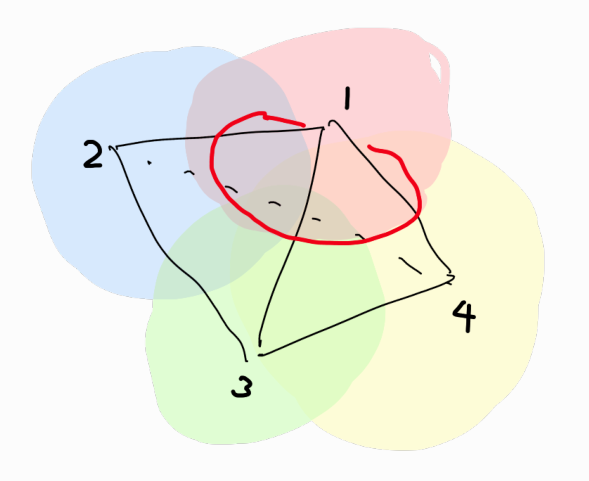
\includegraphics[width=0.62\textwidth]{figures/fig7_1.png}\\[2pt]
{\small 图 7.1：$M$ 上的一个 2-闭链 $C$}
\end{center}

配对 $\langle c_1(P),C\rangle$ 按定义是其中四个三角形上 $c(i,j,k)$ 之和。
在这个特殊情形下，可以让赤道穿过边 12、13、14，使得
$g_{23}(x)=g_{34}(x)=g_{42}(x)=1$。

% [原文 p.107]
取 $g_{12}(x)$、$g_{13}(x)$、$g_{14}(x)$ 为赤道上的粘贴函数 $g(x)$
限制到 $U_{12}$、$U_{13}$、$U_{14}$ 上的部分。为便于计算，可设
$g_{13}(x)=g_{14}(x)=1$，唯一非平凡的地方在 $g_{12}(x)$。
于是唯一非平凡的 $\theta_{ij}(x)$ 是 $\theta_{12}(x)$。
在 $x_3\in U_{123}$ 上，$\theta_{12}(x_3)$ 是不依赖于 $x_3$ 的整数，即 $c(1,2,3)$。
类似地，在 $x\in U_{124}$ 上 $\theta_{12}(x)$ 是不依赖于 $x_4$ 的整数，即 $c(1,2,4)$。
按定义 $c(1,3,4)$ 与 $c(2,3,4)$ 为零。因此配对由
\begin{equation}
\langle c_1(P),C\rangle=c(1,2,3)-c(1,2,4)=\theta_{12}(x_3)-\theta_{12}(x_4),
\tag{7.18}
\end{equation}
给出，它就是 $g(x)$ 在赤道上的缠绕数。

因此它刻画了 $U(1)$-丛 $P$ 在 2-闭链 $C$ 上的拓扑类。
结合此前关于 de Rham 上同调类 $[F/(2\pi)]\in H^2(M,\R)$ 的讨论——它对应丛的某个联络——
我们得到下面这个重要关系：

\begin{proposition}{7.12}
主 $U(1)$-丛 $U(1)\to P\to M$ 的第 1 Chern 类 $c_1(P)$ 满足
\begin{equation}
\langle c_1(P),C\rangle=\int_C\frac{F}{2\pi},
\tag{7.19}
\end{equation}
其中 $F$ 是同一丛上联络的曲率 2-形式。
\end{proposition}

注意，2-形式 $F/(2\pi)$ 用实数定义，却总能积出整数；而 $c_1(P)$ 本质上是用 $\Z$ 定义的。
例如 $S^3/\Z_2$ 上存在主 $U(1)$-丛，其 $F$ 为零但 $c_1(P)$ 非平凡。

\subsection{$SO(3)$ 丛的第 2 Stiefel--Whitney 类}

现在设给定 $SO(3)$-丛 $SO(3)\to P\to M$。它由覆盖块 $U_i$ 与 $U_j$ 之间的转移函数
$g_{ij}(x)\in SO(3)$ 给出。为保持相容性，它们在三重交上满足
$g_{ij}(x)g_{jk}(x)g_{ki}(x)=1$。

我们来看何时能提升为 $SU(2)$-丛 $SU(2)\to\tilde P\to M$。
记投影映射为 $p:SU(2)\to SO(3)$。若存在提升，则会有转移函数
$\tilde g_{ij}(x)\in SU(2)$ 使得
\begin{align}
p(\tilde g_{ij}) &= g_{ij}, \tag{7.20}\\
\tilde g_{ij}(x)\tilde g_{jk}(x)\tilde g_{ki}(x) &= 1. \tag{7.21}
\end{align}

什么时候能找到这样的函数？我们已经假设每个交 $U_{ij}=U_i\cap U_j$ 可缩，
因此可以在每个覆盖块上找到满足上面第一式 (7.20) 的 $\tilde g_{ij}(x)\in SU(2)$。
但第二式 (7.21) 却不一定成立。

假设我们在 $U_{ij}$ 上选好了满足式 (7.20) 的 $\tilde g_{ij}(x)$。此时有
\begin{equation}
p\bigl(\tilde g_{ij}(x)\tilde g_{jk}(x)\tilde g_{ki}(x)\bigr)
=g_{ij}(x)g_{jk}(x)g_{ki}(x)=1,
\tag{7.22}
\end{equation}

% [原文 p.108]
因此
\begin{equation}
\tilde g_{ij}(x)\tilde g_{jk}(x)\tilde g_{ki}(x)=\pm1,
\tag{7.23}
\end{equation}
这里用到了短正合列
\begin{equation}
1\to\Z_2\to SU(2)\to SO(3)\to 1.
\tag{7.24}
\end{equation}
我们用这个量 (7.23) 来定义 $w(i,j,k)$。可以证明 $w(i,j,k)$ 在交换 $i,j,k$ 时反号。

现在有
\begin{equation}
\begin{split}
w(i,j,k)w(i,k,l)&=p(\tilde g_{ij}\tilde g_{jk}\tilde g_{ki})\,p(\tilde g_{ik}\tilde g_{kl}\tilde g_{li})\\
&=p(\tilde g_{ij}\tilde g_{jk}\tilde g_{kl}\tilde g_{li})
\end{split}
\tag{7.25}
\end{equation}
同样有
\begin{equation}
\begin{split}
w(l,i,j)w(l,j,k)&=p(\tilde g_{li}\tilde g_{ij}\tilde g_{jl})\,p(\tilde g_{lj}\tilde g_{jk}\tilde g_{kl})\\
&=p(\tilde g_{li}\tilde g_{ij}\tilde g_{jk}\tilde g_{kl})
\end{split}
\tag{7.26}
\end{equation}
因此
\begin{equation}
w(i,j,k)w(i,k,l)=w(l,i,j)w(l,j,k),
\tag{7.27}
\end{equation}
这意味着 $\delta w=0$。于是 $w$ 是 Čech 2-上闭链，定义了上同调类 $[w]\in H^2(M;\Z_2)$。

若取不同的提升 $\hat g_{ij}(x)\in SU(2)$，则对某个 $f_{ij}\in\Z_2$ 有
$\hat g_{ij}(x)=f_{ij}\tilde g_{ij}(x)$。简单计算可得
\begin{equation}
\hat w(i,j,k)=w(i,j,k)+(\delta f)(i,j,k)
\tag{7.28}
\end{equation}
（这里用了加法记号），因此 $[w]=[\hat w]$。
% [Tutor Note: 原文此处作 $\hat g_{ij}=f_{ij}g_{ij}$ 与 $(\hat w,i,k)=0$，按文义应为 $\hat g_{ij}=f_{ij}\tilde g_{ij}$ 与 $\hat w(i,j,k)=0$；正文照此译，已登记。]

注意，若 $\tilde g_{ij}(x)\in SU(2)$ 满足式 (7.21)，则 $w=0$ 且 $[w]=0$。
反之，若 $[w]=0$，则可选取 $f_{ij}\in\Z_2$，使 $\hat g_{ij}(x)=f_{ij}\tilde g_{ij}(x)$
满足对所有 $i,j,k$ 都有 $\hat w(i,j,k)=0$，也就是说 $\hat g_{ij}(x)\hat g_{jk}(x)\hat g_{ki}(x)=1$。
这说明 $SO(3)$ 丛 $SO(3)\to P\to M$ 提升为 $SU(2)$-丛 $SU(2)\to\tilde P\to M$。

综上，我们得到下面的定理：

\begin{theorem}{7.13}
对 $SO(3)$ 丛 $SO(3)\to P\to M$，可以联系一个上同调类 $w_2(P)\in H^2(M;\Z_2)$，
使得 $w_2(P)=0$ 当且仅当丛 $P$ 提升为 $SU(2)$-丛。这个 $w_2(P)$ 称为 $P$ 的第 2 Stiefel--Whitney 类。
\end{theorem}

\begin{remark}{7.14}
因此，第 2 Stiefel--Whitney 类 $w_2(P)$ 是该丛成为 $SU(2)$-丛的障碍。
\end{remark}

下面给出 $w_2(P)$ 非平凡的两个简单例子。在二维球面 $S^2$ 上，
取北半球 $U_N$ 与南半球 $U_S$ 作为两个覆盖块。$SO(3)$ 丛由赤道到 $SO(3)$ 的映射
$g:S^1\to SO(3)$ 指定。它们由 $\pi_1(SO(3))=\Z_2$ 分类。
$w_2(P)$ 在 $S^2$ 上的配对 $\langle w_2(P),S^2\rangle$，就由 $\Z_2$ 中的这个数给出。

类似地，$S^2$ 上的 $SU(2)$-丛由 $\tilde g:S^1\to SU(2)$ 指定。
映射 $p:SU(2)\to SO(3)$ 给出映射 $\pi_1(SU(2))\to\pi_1(SO(3))$。
由于 $\pi_1(SU(2))=0$，任何 $SU(2)$-丛若看作 $SO(3)$ 丛，都对应
$\pi_1(SO(3))=\Z_2$ 中的平凡类。

% [原文 p.109]
\begin{example}{7.15}
考虑由映射 $g:S^1\to SO(3)$ 给出的 $S^2$ 上的 $SO(3)$ 丛，它对应 $SO(3)$ 中的 $360^\circ$ 旋转，
因此 $[g]\in\pi_1(SO(3))=\Z_2$ 非平凡。这个丛有 $\langle w_2(P),S^2\rangle=1$，不能提升为 $SU(2)$-丛。
% [Tutor Note: 原文此处作 $\langle w_2(P),S^3\rangle$，而该丛定义在 $S^2$ 上，按上下文应为 $S^2$；正文照此译，已登记。]
\end{example}

接着考虑 $T^2$ 上的 $SO(3)$ 丛。把 $T^2$ 看作由 $(s,t)$ 参数化的 $\R^2$ 在等价关系
$(s,t)\sim(s+1,t)\sim(s,t+1)$ 下的商。我们从 $\R^2$ 上的平凡 $\R^3$ 丛 $\R^2\times\R^3$ 出发，
用 $(s,t;x,y,z)$ 参数化。现在作两个等价关系：
\begin{align}
(s,t;x,y,z)&\sim(s+1,t;-x,-y,z), \tag{7.29}\\
(s,t;x,y,z)&\sim(s,t+1;x,-y,-z). \tag{7.30}
\end{align}
前者对应 $SO(3)$ 变换 $\diag(-1,-1,1)$，后者对应 $\diag(1,-1,-1)$。

我们试着把它提升为 $SU(2)$-丛。从 $\R^2\times\C^2$ 出发，用 $(s,t;v)$ 参数化。
$\diag(-1,-1,1)\in SO(3)$ 在 $SU(2)$ 中的提升就是 $\sigma_z$，
而 $\diag(1,-1,-1)\in SO(3)$ 在 $SU(2)$ 中的提升是 $\sigma_x$。
于是我们试着作如下等价关系：
\begin{align}
(s,t;v)&\sim(s+1,t;\sigma_zv), \tag{7.31}\\
(s,t;v)&\sim(s,t+1;\sigma_xv). \tag{7.32}
\end{align}
但这并不相容，因为
\begin{equation}
(s,t;v)\sim(s+1,t;\sigma_zv)\sim(s+1,t+1;\sigma_x\sigma_zv)
\tag{7.33}
\end{equation}
而
\begin{equation}
(s,t;v)\sim(s,t+1;\sigma_xv)\sim(s+1,t+1;\sigma_z\sigma_xv),
\tag{7.34}
\end{equation}
但
\begin{equation}
\sigma_x\sigma_z=-\sigma_z\sigma_x.
\tag{7.35}
\end{equation}
这说明由式 (7.29) 与式 (7.30) 定义的 $T^2$ 上的 $SO(3)$ 丛不能提升为 $SU(2)$-丛，
并且 $\langle w_2(P),T^2\rangle=1\in\{0,1\}=\Z_2$。

\subsection{$SO(n)$ 丛的第 2 Stiefel--Whitney 类}

把 $0\to\Z_2\to SU(2)\to SO(3)\to 0$ 换成
$0\to\Z_2\to Spin(n)\to SO(n)\to 0$，即可得到

\begin{proposition}{7.16}
对 $SO(n)$ 丛 $SO(n)\to P\to M$，可以联系一个示性类，称为第 2 Stiefel--Whitney 类 $w_2(P)$。
这个示性类为零，即 $w_2(P)=0$，当且仅当丛 $P$ 提升为主 $Spin(n)$ 丛。
\end{proposition}

给定流形 $M$，可考虑其切丛 $TM$，它是某个 $O(n)$-丛的相伴向量丛。
若 $M$ 可定向，则 $w_1(TM)=0$，$TM$ 是 $SO(n)$ 丛。
我们可以问它能否进一步提升为 $Spin(n)$。前面已学过，这由 $M$ 的第 2 Stiefel--Whitney 类
$w_2(TM)$ 控制。总结起来，有下面的命题：

% [原文 p.110]
\begin{proposition}{7.17}
流形 $M$ 的第 2 Stiefel--Whitney 类 $w_2(M)$ 为零，当且仅当 $M$ 是 spin 流形。
\end{proposition}

虽然暂时还不能证明，我们有一个重要的定理：

\begin{theorem}{7.18}
任何维数 $\le3$ 的可定向流形都是 spin 流形。
\end{theorem}

\begin{remark}{7.19}
四维存在非 spin 流形，例子是 $\CP^2$。
\end{remark}

把 $U(1)$-丛的 $c_1(P)$ 与 $SO(n)$ 丛的 $w_2(P)$ 的构造再走一遍，会看到两套程序完全平行。
具体说来，前者用了序列
\begin{equation}
0\to\Z\to\R\to U(1)\to 0,
\tag{7.36}
\end{equation}
后者对 $SO(3)$ 用了
\begin{equation}
0\to\Z_2\to SU(2)\to SO(3)\to 0,
\tag{7.37}
\end{equation}
更一般地用了
\begin{equation}
0\to\Z_2\to Spin(n)\to SO(n)\to 0.
\tag{7.38}
\end{equation}

同样的论证可施于任何群的短正合列
\begin{equation}
0\to A\to\Gamma\to G\to 0,
\tag{7.39}
\end{equation}
只要 $A$ 是离散阿贝尔群，即：

\begin{proposition}{7.20}
给定主 $G$-丛 $G\to P\to M$，可以联系一个上同调类 $v_2(P)\in H^2(M;A)$，
使得 $v_2(P)=0$ 当且仅当丛 $P$ 提升为主 $\Gamma$ 丛。
\end{proposition}

\takeaway{次数 2 的示性类：$U(1)$-丛的粘贴函数写成指数后，在三重交上留下整数 2-上闭链，给出第 1 Chern 类 $c_1$，它是曲率积分；$SO(n)$ 丛则有 $w_2$。}

\section{$H^3(M;A)$ 中的一个示性类}

上面讨论过把 $SO(3)$ 丛提升为 $SU(2)$-丛的问题。
在物理里，这是一个自然的问题：考虑旋转群 $SO(3)$ 作用在按旋量变换的波函数上。

在更一般的量子力学语境里，实三维空间也作为二能级系统（量子比特）的 Hermite 算子
$\sigma_{x,y,z}$ 的空间出现。参数空间 $M$ 上的 $\R^3$ 丛，等价地 $SO(3)$ 丛，
可以看成 $M$ 上的一族量子比特，用可观测量描述，或者对偶地用密度矩阵描述。
$M$ 上的 $\C^2$ 丛，等价地 $U(2)$ 丛，也可以看成 $M$ 上的一族量子比特。
我们不禁要问：这两者之间有没有细微差别？

% [原文 p.111]
\subsection{一个例子}

在讨论一般理论之前，先看一个例子。取 $T^2$ 上由上面 (7.29) 与式 (7.30) 的等价关系给出的
$\R^3$ 丛。它不能提升为 $SU(2)$-丛。那它能提升为 $U(2)$ 丛吗？可以。只需取等价关系
\begin{align}
(s,t;v)&\sim(s+1,t;\sigma_zv), \tag{7.40}\\
(s,t;v)&\sim(s,t+1;e^{\pi is}\sigma_xv). \tag{7.41}
\end{align}
这些等价关系现在相容了，因为
\begin{equation}
(s,t;v)\sim(s+1,t;\sigma_zv)\sim(s+1,t+1;e^{\pi i(s+1)}\sigma_x\sigma_zv),
\tag{7.42}
\end{equation}
而
\begin{equation}
(s,t;v)\sim(s,t+1;e^{\pi is}\sigma_xv)\sim(s+1,t+1;e^{\pi is}\sigma_z\sigma_xv).
\tag{7.43}
\end{equation}

给定 $U(2)$ 丛，取行列式 $\det:U(2)\to U(1)$，就得到 $U(1)$-丛。
记它为 $L\to M$，其坐标记为 $w$，则得到等价关系
\begin{align}
(s,t;w)&\sim(s+1,t;w), \tag{7.44}\\
(s,t;w)&\sim(s,t+1;e^{2\pi is}w). \tag{7.45}
\end{align}

这说明，$T^2$ 上提升我们那个 $SO(3)$ 丛的 $U(2)$ 丛，
其行列式 $U(1)$-丛 $L$ 的第 1 Chern 类 $c_1(L)$ 非平凡，且满足 $\langle c_1(L),T^2\rangle=1$。
可以更一般地证明：$T^2$ 上任何提升该 $SO(3)$ 丛的 $U(2)$ 丛，
其第 1 Chern 类都非平凡，并且是奇的：$\langle c_1(L),T^2\rangle=1\bmod 2$。

这个观察可用来构造例子，说明 $M$ 上的 $\R^3$ 丛不能提升为 $U(2)$ 丛。
做法是给 $T^2$ 再加一个坐标 $u\sim u+1$，但用扭曲的等价关系
\begin{equation}
(s,t,u)\sim(s+1,t,u),\quad
(s,t,u)\sim(s,t+1,u),\quad
(s,t,u)\sim(s,-t,u+1).
\tag{7.46}
\end{equation}
这样总的参数空间就是 $S^1$（由 $s$ 参数化）乘上 Klein 瓶（由 $t,u$ 参数化）。
在这个空间上取由上面 (7.29) 与式 (7.30) 给出的 $\R^3$ 丛，但不含 $u$ 依赖。
更确切地说，取等价关系
\begin{align}
(s,t,u;x,y,z)&\sim(s+1,t,u;-x,-y,z), \tag{7.47}\\
(s,t,u;x,y,z)&\sim(s,t+1,u;x,-y,-z), \tag{7.48}\\
(s,t,u;x,y,z)&\sim(s,-t,u+1;x,y,z). \tag{7.49}
\end{align}

要看出这个丛不能提升为 $U(2)$ 丛，可用如下论证。
假设存在提升它的 $U(2)$ 丛。在 $u=u_0$ 固定时，行列式 $U(1)$-丛 $L\to T^2$ 满足
$\langle c_1(L),T^2\rangle=1\bmod 2$，是非平凡的。我们可以连续地改变 $u_0$。
绕 $u$ 圆周走一圈时，$\langle c_1(L),T^2\rangle$ 的值不能变，因为它是整数。
然而，扭曲的等价关系 $(t,u)\sim(-t,u+1)$ 要求：绕 $u$ 圆周走一圈时，$T^2$ 的定向被反转。

% [原文 p.112]
于是绕 $u$ 圆周走一圈时，$\langle c_1(L),T^2\rangle$ 必须变号。这是矛盾，
因此 $T^2\times S^1$ 上的 $\R^3$ 丛不能提升为 $U(2)$ 丛。

下面会说明，之所以不能提升，是因为 $H^3(M;\Z)$ 中存在障碍类。
在 $T^2$ 上 $H^3(T^2;\Z)=0$，障碍自然不存在，
这就解释了为什么 $T^2$ 上的 $SO(3)$ 丛能提升为 $U(2)$ 丛。
但在三维空间上，障碍一般可以非平凡，于是 $SO(3)$ 丛就无法提升为 $U(2)$ 丛。

\subsection{一般理论}

现在问：何时 $SO(3)$ 丛 $SO(3)\to P\to M$ 能提升为 $U(2)$ 丛 $U(2)\to\tilde P\to M$。
照例取足够细的覆盖 $U_i$，使所有非空交 $U_{i_1}\cap U_{i_2}\cap\cdots\cap U_{i_k}$ 可缩。
$SO(3)$ 丛的数据由转移函数 $g_{ij}(x)\in SO(3)$ 给出，它们满足
\begin{equation}
g_{ij}(x)g_{jk}(x)g_{ki}(x)=1.
\tag{7.50}
\end{equation}

前面已讨论过提升为 $SU(2)$ 的问题。为复用那些讨论，把 $U(2)$ 写成
\begin{equation}
U(2)=\frac{U(1)\times SU(2)}{\Z_2},
\tag{7.51}
\end{equation}
其中 $\Z_2\subset U(1)\times SU(2)$ 由 $(-1,-1)$ 生成。的确，任意 $2\times2$ 酉矩阵 $U$ 都可写成
\begin{equation}
U=e^{2\pi i\theta}\tilde U
\tag{7.52}
\end{equation}
其中 $\det\tilde U=1$；但这个分解不唯一，存在歧义
$(e^{2\pi i\theta},\tilde U)\sim(-e^{2\pi i\theta},-\tilde U)$。

$U(2)$ 丛由转移函数 $\tilde g_{ij}(x)\in U(2)$ 指定，它们满足
\begin{equation}
\tilde g_{ij}(x)\tilde g_{jk}(x)\tilde g_{ki}(x)=1.
\tag{7.53}
\end{equation}
利用式 (7.51)，它也可以用对
\begin{equation}
(e^{2\pi i\theta_{ij}(x)},h_{ij}(x))\in U(1)\times SU(2)
\tag{7.54}
\end{equation}
给出，满足
\begin{align}
e^{2\pi i\theta_{ij}(x)}e^{2\pi i\theta_{jk}(x)}e^{2\pi i\theta_{ki}(x)} &= (-1)^{w_{ijk}}, \tag{7.55}\\
h_{ij}(x)h_{jk}(x)h_{ki}(x) &= (-1)^{w_{ijk}}, \tag{7.56}
\end{align}
其中 $w_{ijk}\in\{0,1\}$ 在每个 $U_{ijk}$ 上有定义。

要使这个 $U(2)$ 丛提升给定的 $SO(3)$ 丛，只需
\begin{equation}
p(h_{ij})=g_{ij}.
\tag{7.57}
\end{equation}
这正是上一节反复用到的条件。我们已经知道，条件 (7.56) 说明 $w_{ijk}$ 是 Čech 2-上闭链，
定义了上同调类 $[w]\in H^2(M;\Z_2)$。而条件 (7.55) 还会加上一个额外约束。

% [原文 p.113]
为看出这一点，考虑
\begin{equation}
n_{ijk}(x):=2\bigl(\theta_{ij}(x)+\theta_{jk}(x)+\theta_{ki}(x)\bigr).
\tag{7.58}
\end{equation}
由式 (7.55) 可知，它在每个 $U_{ijk}$ 上其实是常数 $n_{ijk}$，并满足
\begin{equation}
n_{ijk}=w_{ijk}\mod 2.
\tag{7.59}
\end{equation}

$n_{ijk}$ 其实是 Čech 2-上闭链，定义了上同调类 $[n]\in H^2(M;\Z)$。
为看出这一点，注意行列式映射 $\det:U(2)\to U(1)$ 把
$(e^{2\pi i\theta},h)$ 送到 $e^{2\pi i\cdot2\theta}$。因此粘贴函数
$e^{2\pi i\cdot2\theta_{ij}(x)}$ 定义了主 $U(1)$-丛 $U(1)\to L\to M$，
而关系 (7.58) 说明 $n_{ijk}$ 就是给出其第 1 Chern 类 $c_1$ 的 Čech 2-上闭链。
这意味着：$SO(3)$ 丛的上同调类 $w_2(P)\in H^2(M;\Z_2)$，
就是 $U(1)$-丛 $L$ 的上同调类 $c_1(L)\in H^2(M;\Z)$ 的模 2 约化。

反之，设对给定的 $SO(3)$ 丛 $SO(3)\to P\to M$，存在 $U(1)$-丛
$U(1)\to L\to M$，使得 $w_2(P)$ 是 $c_1(L)$ 的模 2 约化。
设 $g_{ij}(x)\in SO(3)$ 是 $P$ 的转移函数，$h_{ij}(x)\in SU(2)$ 是它们在 $SU(2)$ 中的提升，
$e^{2\pi i\cdot2\theta_{ij}(x)}$ 是 $L$ 的粘贴函数，并如上定义 $w$ 与 $n$。
上同调类（而不是上闭链本身）满足 $w_2(P)=c_1(L)$，这说我们有
\begin{equation}
n_{ijk}+(\delta m)_{ijk}=w_{ijk}+(\delta v)_{ijk}\mod 2.
\tag{7.60}
\end{equation}

这意味着可以重取 $\theta_{ij}(x)\mapsto\theta_{ij}(x)+m_{ij}/2$ 与
$h_{ij}(x)\mapsto h_{ij}(x)(-1)^{v_{ij}}$，使关系 (7.59) 严格成立，
从而给出 $SO(3)$ 丛提升为 $U(2)$ 丛的构造。

把到此为止的讨论总结起来，有下面的命题：

\begin{proposition}{7.21}
$SO(3)$ 丛 $SO(3)\to P\to M$ 提升为 $U(2)$ 丛 $U(2)\to\tilde P\to M$，
当且仅当 $w_2(P)\in H^2(M;\Z_2)$ 是某个类 $c\in H^2(M;\Z)$ 的模 2 约化。
\end{proposition}

这里用了这样一个事实：任意类 $c\in H^2(M;\Z)$ 都是 $M$ 上某个主 $U(1)$-丛 $L$ 的第 1 Chern 类。
这一点还没证明，将在下一节证明。

现在需要研究：何时类 $w\in H^2(M;\Z_2)$ 是某个类 $c\in H^2(M;\Z)$ 的模 2 约化。
类 $w$ 由 Čech 2-上闭链 $w_{ijk}\in\Z_2$ 代表。当它是 $c\in H^2(M;\Z)$ 的模 2 约化时，
可以选取提升 $c_{ijk}$，它是 $\Z$ 中的 Čech 2-上闭链。

但这样的上闭链提升并不总是存在。任取 $w_{ijk}$ 在 $\Z$ 中的提升 $c_{ijk}$。
它是一个上链，却不一定上闭。下面研究它上闭性的失效。我们有
\begin{equation}
(\delta c)_{ijkl}=c_{jkl}-c_{ikl}+c_{ijl}-c_{ijk}
\tag{7.61}
\end{equation}
它总是偶数，因为
\begin{equation}
=w_{ijk}+w_{jkl}+w_{kli}+w_{lij}=(\delta w)_{ijkl}=0\mod 2.
\tag{7.62}
\end{equation}

于是定义
\begin{equation}
d_{ijkl}=\frac12\bigl(c_{jkl}-c_{ikl}+c_{ijl}-c_{ijk}\bigr)\in\Z.
\tag{7.63}
\end{equation}

% [原文 p.114]
这是 Čech 3-上闭链，因为
\begin{equation}
(\delta d)_{ijklm}=\frac12(\delta\delta c)_{ijklm}=0.
\tag{7.64}
\end{equation}

于是我们定义了类 $[d]\in H^3(M;\Z)$。按构造，若 $w_{ijk}$ 有上闭链提升 $c_{ijk}$，
这个类就为零。

反之，若这个类为零，则有一个上链 $d=\delta e$。这时把 $c_{ijk}+2e_{ijk}$ 取作
$w_{ijk}$ 的新提升；按构造它是上闭链。

这样就知道：类 $w\in H^2(M;\Z_2)$ 是某个类 $c\in H^2(M;\Z)$ 的模 2 约化，
当且仅当上面构造的类 $[d]\in H^3(M;\Z)$ 为零。
这个构造看起来有些凑巧，我们把它稍作推广。

取阿贝尔群的短正合列
\begin{equation}
0\to A\to B\to C\to 0.
\tag{7.65}
\end{equation}
上面讨论的情形对应
\begin{equation}
0\to\Z\xrightarrow{\times2}\Z\xrightarrow{\bmod 2}\Z_2\to 0.
\tag{7.66}
\end{equation}

我们来研究：何时类 $w\in H^2(M;C)$ 来自某个类 $c\in H^2(M;B)$。
为此取 $w$ 的上闭链代表 $w_{ijk}\in C$，再任取提升 $c_{ijk}\in B$。
按构造，$(\delta c)_{ijkl}$ 落在 $B\to C$ 的核里，即在 $A\to B$ 的像里。因此可写成
\begin{equation}
(\delta c)_{ijkl}=d_{ijkl}
\tag{7.67}
\end{equation}
其中 $d_{ijkl}\in A$。这定义了 Čech 3-上闭链 $[d]\in H^3(M;A)$。
类 $w\in H^2(M;C)$ 来自某个类 $c\in H^2(M;B)$，当且仅当 $[d]\in H^3(M;A)$ 为零。总结如下：

\begin{definition}{7.22}
上面构造的同态 $\beta:H^2(M;B)\to H^3(M;A)$，
与短正合列 $0\to A\to B\to C\to 0$ 相伴，称为 Bockstein 同态。
\end{definition}

\begin{proposition}{7.23}
类 $w\in H^2(M;C)$ 来自某个类 $c\in H^2(M;B)$，
当且仅当其 Bockstein $\beta(w)\in H^3(M;A)$ 为零。
% [Tutor Note: 原文此处作 $\beta(w)\in H^2(M;A)$，按 $\beta:H^2(M;B)\to H^3(M;A)$ 应为 $H^3(M;A)$；正文照此译，已登记。]
\end{proposition}

回到 $SO(3)$ 丛能否提升为 $U(2)$ 丛的问题，现在有下面的命题：

\begin{proposition}{7.24}
$SO(3)$ 丛 $SO(3)\to P\to M$ 提升为 $U(2)$ 丛 $U(2)\to\tilde P\to M$，
当且仅当 Bockstein $\beta(w_2(P))\in H^3(M;\Z)$ 为零。
\end{proposition}

\begin{remark}{7.25}
因此，次数 3 的类 $\beta(w_2(P))$ 是该 $SO(3)$ 丛提升为 $U(2)$ 丛的障碍。
$\beta(w_2(P))$ 也称为该 $SO(3)$ 丛的整第 3 Stiefel--Whitney 类，记作 $W_3(P)$。
更常见的第 3 Stiefel--Whitney 类 $w_3(P)\in H^3(M;\Z_2)$ 是 $W_3(P)$ 的模 2 约化。
\end{remark}

% [原文 p.115]
\begin{question}{7.26}
这里只讨论了把 $SO(3)$ 丛提升为 $U(2)$ 丛的情形，
它对应二能级系统（即量子比特）的密度矩阵问题。
如果改考虑 $n$ 能级系统，对称性 $U(n)$ 作用在 希尔伯特空间 $\C^n$ 上，
而作用在密度矩阵上的对称性是
\begin{equation}
PU(n):=\frac{U(n)}{U(1)}=\frac{U(1)\times SU(n)}{\Z_n},
\tag{7.68}
\end{equation}
其中 $\Z_n$ 以 $(e^{2\pi i/n},e^{-2\pi i/n})$ 嵌入 $U(1)\times SU(n)$，那会怎样？
\end{question}

\takeaway{次数 3 的障碍：把模 2 约化的 2-上闭链提升到整数上链，提升失效由 Bockstein 同态 $\beta$ 量度；$\beta(w_2)$ 就是整第 3 Stiefel--Whitney 类 $W_3$，它挡住提升为 $U(2)$ 丛。}

\section{分类空间}

\subsection{主 $G$-丛的情形}

下面引进主 $G$-丛的分类空间这一概念。

\begin{definition}{7.27}
主 $G$ 纤维丛 $G\to E\to B$ 的底空间 $B$，若满足对任意 $k$ 都有 $\pi_k(E)=0$，
则称为分类空间，记作 $BG$。整个纤维丛记作 $G\to EG\to BG$。
\end{definition}

\begin{remark}{7.28}
这样的分类丛 $EG\to BG$ 是否存在、存在时是否唯一，并不显然。
结果表明，这样的 $EG\to BG$ 总是存在，并且在同伦意义下唯一。
\end{remark}

例如回忆 $U(1)$ 纤维丛 $U(1)\to S^{2n+1}\to\CP^n$。
它在 $k<2n+1$ 时满足 $\pi_k(S^{2n+1})=0$。
因此适当取极限 $n\to\infty$，就得到

\begin{example}{7.29}
$BU(1)=\CP^\infty$。
% [Tutor Note: 原文此处作 $\CP^n$，而前文已取极限 $n\to\infty$，按文义应为 $\CP^\infty$；正文照此译，已登记。]
\end{example}

分类空间这一概念的重要性来自下面的定理：

\begin{theorem}{7.30}
任意空间 $X$ 上的主 $G$-丛 $E\to X$，都可由映射 $f:X\to BG$ 拉回 $EG\to BG$ 得到。
而且，$X$ 上主 $G$-丛的等价类与映射 $f:X\to BG$ 的同伦类一一对应。
\end{theorem}

\begin{proof}[证明概要（定理 7.30）]
我们引用过定理 4.61：同伦的两个映射 $f,f':X\to Y$ 在拉回下给出等价的丛。
所以只需说明：由主 $G$-丛 $G\to E\to X$ 能构造出映射 $f:X\to BG$。
设 $X$ 取 CW 复形的结构。我们归纳地构造映射。
在 $0$-骨架 $X_0$ 上，显然可以构造映射 $f_0:X_0\to BG$，使拉回是 $X_0$ 上的 $G$-丛。
现设已构造到 $f:X_k\to BG$，要延拓为 $f:X_{k+1}\to BG$。
为此只需逐个胞腔处理。于是要做的事是：给定主 $G$-丛 $E\to B^{k+1}$，
以及映射 $f:S^k\to BG$，使拉回 $f^*(EG)\to S^k$ 与 $E$ 在边界上的限制一致，
构造映射 $f:B^k\to BG$，使上述结论成立。

% [原文 p.116]
为此注意，任何丛 $G\to E\to B^{k+1}$ 都拓扑平凡，因此它在边界 $S^k$ 上的限制也拓扑平凡。
这说明它有截面 $S^k\to E$。利用 $E\to S^k$ 与 $f^*(EG)\to S^k$ 的等价性，
可把这个截面看成映射 $S^k\to EG$。由假设 $\pi_k(EG)=0$，可把它延拓为 $B^{k+1}\to EG$。
再与投影 $EG\to BG$ 复合，就把映射延拓到了 $B^{k+1}\to BG$。
验证所得映射满足要求，是例行公事。
\end{proof}

\begin{remark}{7.31}
$BU(1)=\CP^\infty$ 是无穷维的，也许让你不安。但上面的证明表明：要分类维数至多 $n$ 的空间 $X$
上的主 $G$-丛，只需 $k<n$ 时 $\pi_k(BG)=0$。因此，对理论物理学家的大部分用途，
取充分大的有限 $n$ 的 $\CP^n$ 就够了。不过取 $n\to\infty$ 确实能让定理的陈述更简洁，
所以习惯上采用无穷维的分类空间。
\end{remark}

分类空间的存在性是一个非平凡的定理：

\begin{theorem}{7.32}
对任何群 $G$，分类丛 $G\to EG\to BG$ 都存在。
\end{theorem}

其证明我们无暇展开。但同伦意义下的唯一性可由上面的定理简单推出：

\begin{proposition}{7.33}
两个分类丛 $EG\to BG$ 与 $E'G\to B'G$ 在同伦意义下相同。
\end{proposition}

\begin{proof}[证明概要]
由上面的定理，有映射 $f:BG\to B'G$ 与 $g:B'G\to BG$，使两个丛互为拉回。
特别地，$g\circ f:BG\to BG$ 把丛 $EG\to BG$ 拉回自身。因此 $g\circ f$ 同伦于恒等映射。
\end{proof}

\subsection{上同调群的情形}

上同调群也有分类空间。为此需要一些准备。

\begin{definition}{7.34}
设 $A$ 是阿贝尔群。若空间 $X$ 满足 $\pi_k(X)=A$，且 $\ell\neq k$ 时 $\pi_\ell(X)=0$，
则称 $X$ 为 $K(A,k)$ 空间，也称为 Eilenberg--Mac Lane 空间。
\end{definition}

还需要：

\begin{theorem}{7.35}
对任意 $A$ 与 $k$，$K(A,k)$ 空间存在，且在同伦意义下唯一。
\end{theorem}

例如再考虑 $U(1)\to S^{2n+1}\to\CP^n$。由同伦长正合列可知，
$\pi_k(\CP^n)$ 只在 $\pi_2=\Z$ 与 $\pi_{2n+1}=\Z$ 处非零。适当取极限 $n\to\infty$，就得到

\begin{example}{7.36}
$K(\Z,2)=\CP^\infty$。
\end{example}

Eilenberg--Mac Lane 空间 $K(A,k)$ 的重要性在于下面这一点。

% [原文 p.117]
\begin{theorem}{7.37}
对任意空间 $X$，上同调类 $a\in H^k(X;A)$ 与映射 $f:X\to K(A,k)$ 的同伦类一一对应。
\end{theorem}

\begin{proof}[证明概要]
这里只给出由上同调类 $a$ 构造 $f$ 的做法。设 $X$ 取单纯复形的结构，归纳地进行。
取代表 $a$ 的显式上闭链 $a(\sigma)$。由于 $\ell<k$ 时 $\pi_\ell(K(A,k))=0$，
可以取映射 $f:X_{k-1}\to K(A,k)$，它与恒等映射同伦。
% [Tutor Note: 原文此处作 $\pi_\ell(X)=0$，而 $X$ 是任意的，按上下文应为 $\pi_\ell(K(A,k))=0$；正文照此译，已登记。]
对每个 $k$-单形 $\sigma$，把它看作 $B^k$。其边界已被映到基点。于是只需指定映射
$S^k\to K(A,k)$。这里取代表元素 $a(\sigma)\in A=\pi_k(K(A,k))$ 的映射。
现在有了映射 $f:X_k\to K(A,k)$。要把它延拓为 $f:X_{k+1}\to K(A,k)$，
需要对每个 $(k+1)$-单形 $\sigma\simeq B^{k+1}$，把已给的映射 $S^k\to K(A,k)$
延拓为 $B^{k+1}\to K(A,k)$。这恰因 $a(\sigma)$ 是上闭链而可行。
\end{proof}

我们已经看到 $\CP^\infty$ 既是 $BU(1)$ 又是 $K(\Z,2)$。因此：

\begin{theorem}{7.38}
对任意 $X$，$X$ 上主 $U(1)$-丛与 $H^2(X;\Z)$ 中的上同调类一一对应。
\end{theorem}

若把上面两个证明的细节对照起来，你会发现这样得到的上同调类，
正是你出发时那个 $U(1)$-丛的 $c_1$。

这可以用更形式化的方式论证。为此回到一般情形。

\begin{proposition}{7.39}
$H^k(K(A,k);A)=\Hom(A,A)$。
\end{proposition}

\begin{proof}[证明概要]
这由 Hurewicz 定理与万有系数定理推出。
\end{proof}

\begin{definition}{7.40}
$\iota\in H^k(K(A,k);A)$ 是 $\Hom(A,A)\simeq H^k(K(A,k);A)$ 中的恒等映射。
\end{definition}

上面的定理 7.37 可以细化如下：

\begin{theorem}{7.41}
$f:X\to K(A,k)$ 与 $f(\iota)\in H^k(X;A)$ 的对应是双射。
\end{theorem}

现在，在 $BU(1)=\CP^\infty$ 上，$H^2(\CP^\infty;\Z)=\Hom(\Z,\Z)=\Z$，
而丛 $U(1)\to S^{2\infty+1}\to\CP^\infty$ 的 $c_1$ 就是生成元 $\iota$。
由于拉回的 $c_1$ 就是 $c_1$ 的拉回，我们就把定理 7.38 细化为

\begin{theorem}{7.42}
对任意 $X$，主 $U(1)$-丛 $U(1)\to P\to X$ 与其第 1 Chern 类 $c_1(P)\in H^2(X;\Z)$ 的对应，
给出 $X$ 上主 $U(1)$-丛的等价类与 $H^2(X;\Z)$ 中上同调类之间的双射。
\end{theorem}

\begin{corollary}{7.43}
$H^2(X;\Z)$ 中任何上同调类都是某个主 $U(1)$-丛的第 1 Chern 类。
\end{corollary}


% 注：第 7 章的 \\section{§7.5} 末段（p.118 上半、式 (7.69)–(7.71)）及其 \\takeaway 与
% \\chapterreview 按整页切块写在本目录的 ch08.tex 开头（原书 p.118 整页归 ch08 块），
% 并非本章缺漏；整书合并后顺序正确。
